\documentclass{beamer}
\mode<presentation> {

% The Beamer class comes with a number of default slide themes
% which change the colors and layouts of slides. Below this is a list
% of all the themes, uncomment each in turn to see what they look like.
\usepackage{graphicx}
\usepackage{xspace}
%\usetheme{default}
%\usetheme{AnnArbor}
%\usetheme{Antibes}
%\usetheme{Bergen}
%\usetheme{Berkeley}
%\usetheme{Berlin}
%\usetheme{Boadilla}
%\usetheme{CambridgeUS}
%\usetheme{Copenhagen}
%\usetheme{Darmstadt}
%\usetheme{Dresden}
%\usetheme{Frankfurt}
%\usetheme{Goettingen}
%\usetheme{Hannover}
%\usetheme{Ilmenau}
%\usetheme{JuanLesPins}
%\usetheme{Luebeck}
\usetheme{Madrid}
%\usetheme{Malmoe}
%\usetheme{Marburg}
%\usetheme{Montpellier}
%\usetheme{PaloAlto}
%\usetheme{Pittsburgh}
%\usetheme{Rochester}
%\usetheme{Singapore}
%\usetheme{Szeged}
%\usetheme{Warsaw}

% As well as themes, the Beamer class has a number of color themes
% for any slide theme. Uncomment each of these in turn to see how it
% changes the colors of your current slide theme.

%\usecolortheme{albatross}
%\usecolortheme{beaver}
%\usecolortheme{beetle}
%\usecolortheme{crane}
%\usecolortheme{dolphin}
%\usecolortheme{dove}
%\usecolortheme{fly}
%\usecolortheme{lily}
%\usecolortheme{orchid}
%\usecolortheme{rose}
%\usecolortheme{seagull}
%\usecolortheme{seahorse}
%\usecolortheme{whale}
%\usecolortheme{wolverine}

%\setbeamertemplate{footline} % To remove the footer line in all slides uncomment this line
%\setbeamertemplate{footline}[page number] % To replace the footer line in all slides with a simple slide count uncomment this line

%\setbeamertemplate{navigation symbols}{} % To remove the navigation symbols from the bottom of all slides uncomment this line
}

\usepackage{graphicx} % Allows including images
\usepackage{booktabs} % Allows the use of \toprule, \midrule and \bottomrule in tables

%----------------------------------------------------------------------------------------
%	TITLE PAGE
%----------------------------------------------------------------------------------------

\title[Short title]{MedicBot: A New Virtual Assistance for the Children with Auditory Processing Disorder } % The short title appears at the bottom of every slide, the full title is only on the title page

\author{Do Dung Vu} % Your name
\institute[ETS] % Your institution as it will appear on the bottom of every slide, may be shorthand to save space
{
Département de génie logiciel et des TI \\ % Your institution for the title page
\medskip
\textit{do-dung.vu.1@ens.etsmtl.ca } % Your email address
}
\date{\today} % Date, can be changed to a custom date

\begin{document}

\begin{frame}
\titlepage % Print the title page as the first slide
\end{frame}

\begin{frame}
\frametitle{Overview} % Table of contents slide, comment this block out to remove it
\tableofcontents % Throughout your presentation, if you choose to use \section{} and \subsection{} commands, these will automatically be printed on this slide as an overview of your presentation
\end{frame}

%----------------------------------------------------------------------------------------
%	PRESENTATION SLIDES
%----------------------------------------------------------------------------------------

%------------------------------------------------
\section{Introduction} % Sections can be created in order to organize your presentation into discrete blocks, all sections and subsections are automatically printed in the table of contents as an overview of the talk
%------------------------------------------------

\subsection{} % A subsection can be created just before a set of slides with a common theme to further break down your presentation into chunks

\begin{frame}
\frametitle{Introduction}
\begin{itemize}
	\item Auditory processing is defined as what we do with what we hear \footnote{Katz  \&  Tillery,  2004}
	\item Auditory Processing Disorder (APD) is a condition where someone has normal hearing, but the auditory system does not faithfully bring information to the brain \footnote{https://www.sac-oac.ca}
	\item \textbf{Approximate 2-4\% of school age children have APD} \footnote{http://www.ementalhealth.ca/}
\end{itemize}

\end{frame}

\begin{frame}
\frametitle{Objectives}
Propose an AI model (virtual assitance) to assit in diagnosing, monitoring, and training of the children with APD problem
\begin{itemize}
	\item Diagnose APD symptoms based on conversation with the considered children
	\item Create a Training Therapy Model Assitance (adaptable)
	\item Build the Reinforcement Learining (RL) Model to monitor the progress of APD treatment
\end{itemize}

\end{frame}
%------------------------------------------------
\section{Methodology } % Sections can be created in order to organize your presentation into discrete blocks, all sections and subsections are automatically printed in the table of contents as an overview of the talk
%------------------------------------------------
\subsection{} % A subsection can be created just before a set of slides with a common theme to further break down your presentation into chunks

\begin{frame}
	\frametitle{Methodology}
	\begin{itemize}
		\item Analysis  the  given  APD  symptoms  by  speech  	
		recognition  based  on  Deep  learning
		
		\item \color{gray} Analysis  the  given  APD  therapy  and  recommend  the
		
		treatment  to  the  APD  children.  Apply  a  natural  language
		
		processing  (NLP)  to  generate  sentences  and  exploit  Deep
		
		learning  to  understand  the  context  of  the  speech
		
		\item Monitoring  the  process  of  APD  treatment  by  using  speech 	and  behavior  recognition  and  analysis  based  on  Deep
		
		learning
	\end{itemize}

\end{frame}
%------------------------------------------------
\section{Techniques } % Sections can be created in order to organize your presentation into discrete blocks, all sections and subsections are automatically printed in the table of contents as an overview of the talk
%------------------------------------------------


\begin{frame}
	\frametitle{Techniques}
	
	\begin{columns}[T]
		\begin{column}{.5\textwidth}
			\begin{itemize}
				\item Convert text to speech
			\end{itemize}
		\end{column}
		\begin{column}{.5\textwidth}
			
			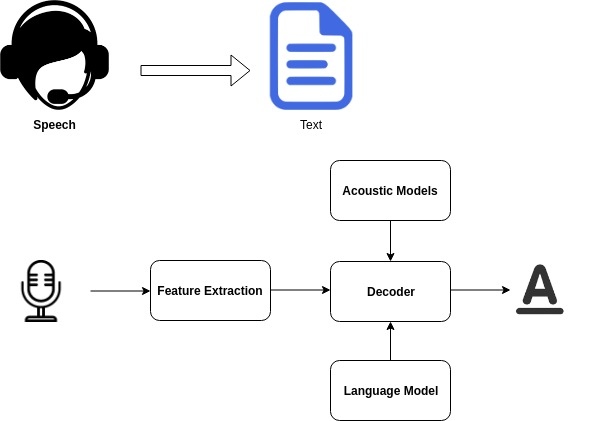
\includegraphics[width=65mm]{f1.jpg}
			
		\end{column}
	\end{columns}

\end{frame}

%------------------------------------------------



\begin{frame}
	\frametitle{Techniques}
	\begin{columns}[T]
		\begin{column}{.5\textwidth}
					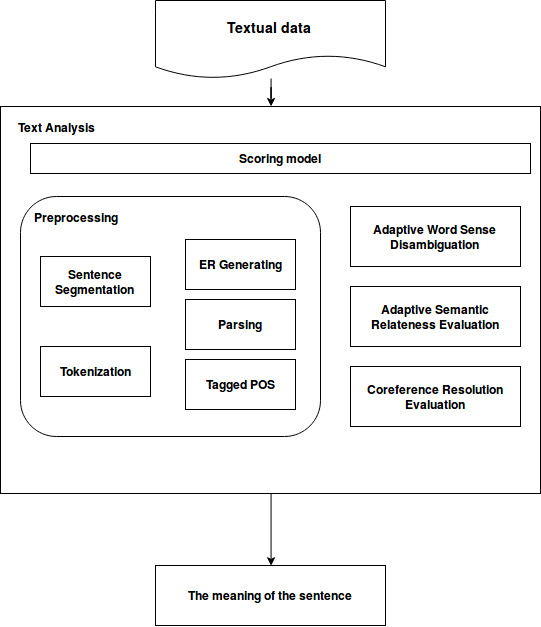
\includegraphics[width=55mm]{f21.jpg}
		\end{column}
		\begin{column}{.5\textwidth}
			
		\begin{itemize}
		\item Step 1: Get the raw text data from the user conversation
		\item Step 2: Process text go extract and compute the score of features based 
		\item Step 3: Adapt word sense disambiguation
		\item Step 4: Evalue the semantic relateness and coreference resolution
		\item Step 5: Get the meaning of the sentence
	\end{itemize}
			
		\end{column}
	\end{columns}

\end{frame}
\begin{frame}
\frametitle{Techniques}
\textbf{Preprocessing} 
\begin{columns}[T]
	\begin{column}{.3\textwidth}
		
	\end{column}
	\begin{column}{.7\textwidth}
		
		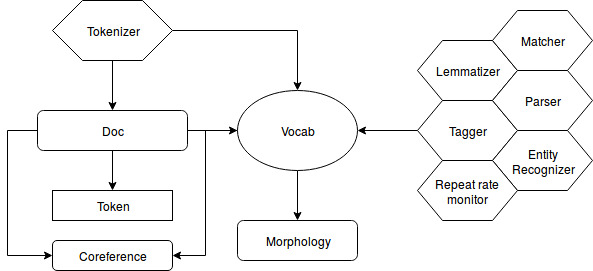
\includegraphics[width=65mm]{f5.jpg}
		
	\end{column}
\end{columns}

\end{frame}

\begin{frame}
\frametitle{Techniques}
\textbf{Scoring model} 
\begin{columns}[T]
	\begin{column}{.3\textwidth}
	
	\end{column}
	\begin{column}{.7\textwidth}
		
		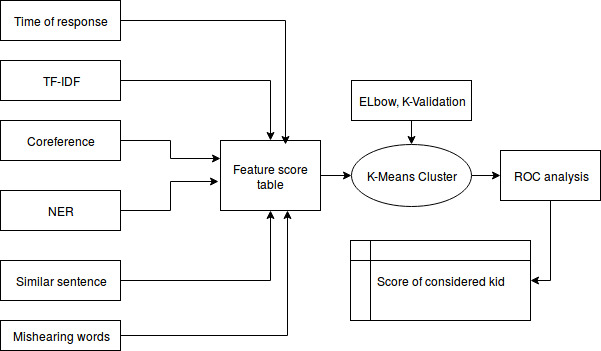
\includegraphics[width=65mm]{f6.jpg}
		
	\end{column}
\end{columns}

\end{frame}
%------------------------------------------------
\begin{frame}
	\frametitle{Methodology}
	\begin{itemize}
		\item \textcolor{gray}{Analysis  the  given  APD  symptoms  by  speech  
		recognition  based  on  Deep  learning}
		\item Analysis  the  given  APD  therapy  and  recommend  the
			
			treatment  to  the  APD  children.  Apply  a  natural  language
			
			processing  (NLP)  to  generate  sentences  and  exploit  Deep
			
			learning  to  understand  the  context  of  the  speech
		
		\item \textcolor{gray} {Monitoring  the  process  of  APD  treatment  by  using  speech 	and  behavior  recognition  and  analysis  based  on  Deep learning}
	
	\end{itemize}

\end{frame}
\begin{frame}
	\frametitle{Techniques}
	
		\begin{column}{.3\textwidth}
	
	\end{column}
	\begin{column}{.7\textwidth}
		
			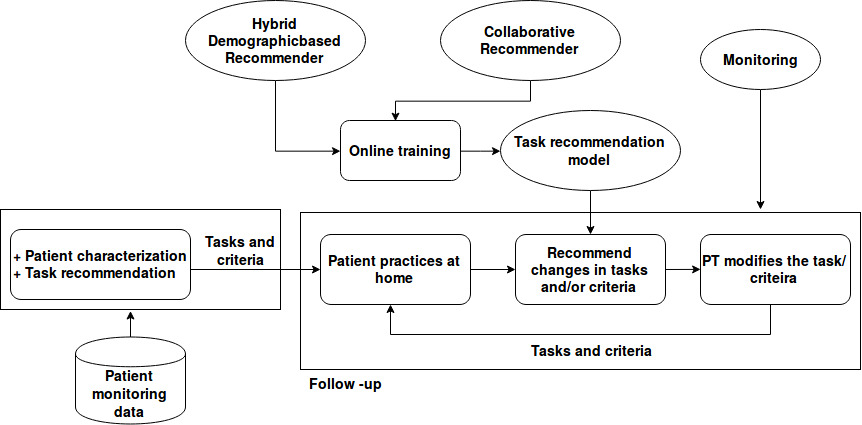
\includegraphics[width=65mm]{f3(1).jpg}
		
	\end{column}
\end{frame}

%------------------------------------------------
\begin{frame}
	\frametitle{Methodology}
	\begin{itemize}
		\item \textcolor{gray}{Analysis  the  given  APD  symptoms  by  speech  
			recognition  based  on  Deep  learning}
		\item \textcolor{gray} {Analysis  the  given  APD  therapy  and  recommend  the 	treatment  to  the  APD  children.  Apply  a  natural  language 	processing  (NLP)  to  generate  sentences  and  exploit  Deep 	learning  to  understand  the  context  of  the  speech}
		
		\item Monitoring  the  process  of  APD  treatment  by  using  speech 	and  behavior  recognition  and  analysis  based  on  Deep learning
		
	\end{itemize}

\end{frame}

\begin{frame}
	\frametitle{Techniques}
	
	\begin{column}{.7\textwidth}
			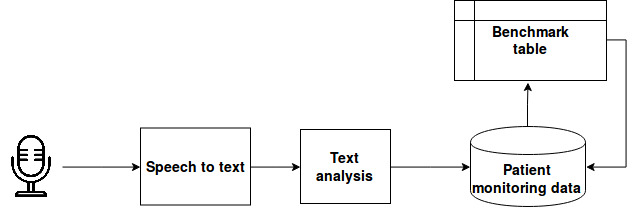
\includegraphics[width=65mm]{f4.jpg}
	\end{column}
	\begin{column}{.3\textwidth}
		
	
		
	\end{column}
\end{frame}
%------------------------------------------------



%------------------------------------------------



\end{document}